% CPE333 Operating Systems - PS6 Virtual Memory
% Overleaf-ready: upload main.tex + figures/ into one Overleaf project, compiler pdfLaTeX
\documentclass[a4paper,11pt]{article}
\usepackage[utf8]{inputenc}
\usepackage[T1]{fontenc}
\usepackage{lmodern}
\usepackage[a4paper,margin=2.2cm]{geometry}
\usepackage{graphicx}
\graphicspath{{figures/}}
\usepackage{float}
\usepackage{caption}
\usepackage{booktabs}
\usepackage{hyperref}
\usepackage{xcolor}
\usepackage{listings}
\hypersetup{colorlinks=true,linkcolor=blue!60!black,citecolor=blue!60!black,urlcolor=blue!60!black}
\lstset{
  basicstyle=\ttfamily\small,
  backgroundcolor=\color{gray!8},
  frame=single,
  breaklines=true,
  columns=fullflexible,
  keepspaces=true,
  showstringspaces=false,
  captionpos=b
}
\title{CPE333 Operating Systems\\Problem Session 6: Virtual Memory}
\author{Group: \_\_\_ \\ Member 1: Thanaboon Tikaew -- 67070501021 \\ Member 2: Chanon Lhumsa-ard -- 67070501059 \\ Member 3: Siriwan Yindeepot -- 67070501075}

\begin{document}
\maketitle
\begin{center}
\fbox{\parbox{0.92\linewidth}{\textbf{Environment used in this report:} Ubuntu 26.04 LTS on WSL2 (7.4\,GiB RAM, 2.0\,GiB swap on \texttt{/dev/sdc}), Windows 11 Home Single Language (16\,GB RAM: 2$\times$8\,GB Kingston 5600). Scripts: \texttt{scripts/linux\_collect.sh}, \texttt{scripts/swap\_demo.sh}, \texttt{scripts/windows\_collect.ps1}. Raw outputs: \texttt{outputs/}. Figures: \texttt{report/figures/}.}}
\end{center}


\section{Virtual memory concept}
\subsection{How virtual memory is implemented in modern Linux and Windows}
Each process gets its own private virtual address space. The MMU translates virtual pages to physical frames via multi-level page tables (4 levels on x86-64, 5 with LA57). Unreferenced or cold pages are kept on secondary storage and brought in on demand (demand paging); a page fault triggers the fault handler to load the page.

\textbf{Linux (modern kernels 5.x/6.x).} Per-process 128\,TiB user space on x86-64; page cache unifies file I/O and memory; swap can be a dedicated partition or a swap file (\texttt{mkswap}/\texttt{swapon}), plus \texttt{zram}/\texttt{zswap} compressed swap; memory overcommit is allowed with heuristics and the OOM-killer reclaims under pressure; page replacement is an LRU-inspired CLOCK/folio-based reclaim with active/inactive lists; \texttt{cgroups} enforce per-group limits.

\textbf{Windows 10/11.} Per-process 128\,TiB user space; paging file \texttt{C:\textbackslash pagefile.sys} (system-managed, can be split across volumes) plus a separate compressed memory store (Memory Compression); each process has a \textit{working set} (resident pages) with min/max trims; system-wide page lists: Zeroed, Free, Standby (cached, repurposable), Modified (dirty, lazily written), Bad; commit charge vs.\ commit limit enforces \texttt{RAM + pagefiles} accounting; SuperFetch/SysMain prefetches.

\begin{table}[H]
\centering
\caption{Linux vs.\ Windows virtual memory (simplified).}
\begin{tabular}{@{}lll@{}}
\toprule
Aspect & Linux & Windows \\
\midrule
Address space & per-process virtual, 4/5-level tables & per-process virtual, 4-level tables \\
Backing store & swap partition/file, zram/zswap & pagefile.sys + compressed store \\
Page-in & demand paging on fault & demand paging on fault \\
Replacement & active/inactive LRU reclaim & working-set trimming + standby/modified lists \\
Overcommit & allowed (heuristic/strict), OOM-killer & commit limit = RAM + pagefiles, fail early \\
Monitoring & \texttt{free}, \texttt{vmstat}, \texttt{/proc/meminfo} & Resource Monitor, \texttt{Get-Counter}, Task Manager \\
\bottomrule
\end{tabular}
\end{table}

\subsection{Increase / decrease swap space on Linux (step-by-step)}
Tested on WSL2 Ubuntu 26.04. The same commands work on bare-metal Ubuntu; on WSL the underlying swap partition (\texttt{/dev/sdc}, 2\,GiB) is provisioned by WSL, so a swap \textit{file} demo is the portable way. \texttt{swapon}/\texttt{swapoff} require \texttt{sudo} (password prompt).

Initial state (real capture from this machine):
\begin{lstlisting}[caption={Before: free and swapon}]
$ free -h
               total        used        free      shared  buff/cache   available
Mem:           7.4Gi       1.1Gi       3.6Gi        51Mi       2.9Gi       6.3Gi
Swap:          2.0Gi          0B       2.0Gi
$ swapon --show
NAME      TYPE      SIZE USED PRIO
/dev/sdc  partition   2G   0B   -2
\end{lstlisting}

Steps to \textbf{increase} swap by 1\,GiB (script \texttt{scripts/swap\_demo.sh}):
\begin{lstlisting}[caption={Increase swap}]
# 1. create a 1 GiB file
fallocate -l 1G ~/swapfile_demo && ls -lh ~/swapfile_demo
# 2. only root may read it
chmod 600 ~/swapfile_demo
# 3. format as swap
sudo mkswap ~/swapfile_demo
# 4. enable it
sudo swapon ~/swapfile_demo
# 5. verify
free -h; swapon --show
\end{lstlisting}
Expected after-step: \texttt{free -h} shows \texttt{Swap: 3.0Gi}, and \texttt{swapon --show} lists both \texttt{/dev/sdc} and \texttt{\textasciitilde/swapfile\_demo}. Non-privileged \texttt{mkswap} was verified on this machine (64\,MiB test file formats correctly as ``Linux swap file, 4k page size'').

Steps to \textbf{decrease} (remove) swap:
\begin{lstlisting}[caption={Decrease swap}]
sudo swapoff ~/swapfile_demo
sudo rm -f ~/swapfile_demo
free -h; swapon --show   # back to 2.0Gi, only /dev/sdc
\end{lstlisting}
Persistent across reboot (bare metal): add to \texttt{/etc/fstab}:
\begin{lstlisting}
~/swapfile_demo none swap sw 0 0
\end{lstlisting}
On WSL2, persistent host-level swap is instead set in Windows \texttt{\%UserProfile\%/.wslconfig} (\texttt{memory}, \texttt{swap} keys), then \texttt{wsl --shutdown} and restart.

\begin{figure}[H]\centering
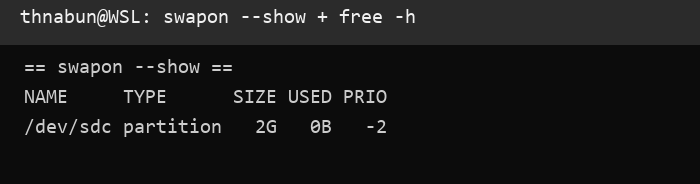
\includegraphics[width=0.9\linewidth]{swapon.png}
\caption{\texttt{swapon --show} on this machine (2\,GiB \texttt{/dev/sdc} partition).}
\end{figure}

\section{Linux VM monitoring}
\subsection{\texttt{free}}
\begin{figure}[H]\centering
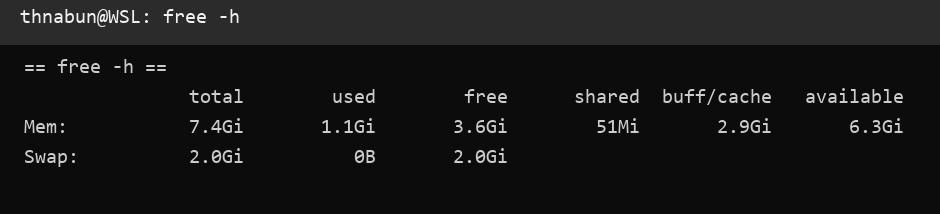
\includegraphics[width=0.95\linewidth]{free_h.png}
\caption{\texttt{free -h} capture.}
\end{figure}
Output fields: \texttt{total} = installed RAM/swap; \texttt{used} = total $-$ free $-$ buff/cache; \texttt{free} = completely idle; \texttt{shared} = tmpfs/shmem; \texttt{buff/cache} = kernel buffers + page cache reclaimable; \texttt{available} = estimate for new processes without swapping (accounts reclaimable cache); \texttt{Mem} row = physical RAM; \texttt{Swap} row = swap space.

\textbf{Paragraph summary of values:} On this WSL machine physical memory totals 7.4\,GiB, of which 1.1\,GiB is used, 3.6\,GiB is fully free, 51\,MiB is shared, 2.9\,GiB sits in buffers/cache, leaving 6.3\,GiB available to new workloads without swapping; swap totals 2.0\,GiB and is entirely free (0\,B used), consistent with \texttt{swapon --show} reporting a 2\,GiB \texttt{/dev/sdc} partition at 0\,B used.

\subsection{Two useful \texttt{free} arguments}
\texttt{free --help} offers unit, layout, and repeat options.
\begin{figure}[H]\centering
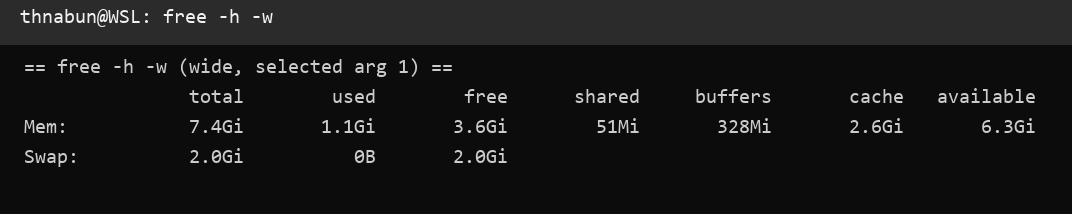
\includegraphics[width=0.95\linewidth]{free_wide.png}
\caption{\texttt{free -h -w} (wide: splits buff/cache into buffers/cache).}
\end{figure}
\textbf{(1) \texttt{-w / --wide}:} splits \texttt{buff/cache} into separate \texttt{buffers} and \texttt{cache} columns. Sample: \texttt{free -h -w} shows 328\,MiB buffers and 2.6\,GiB cache instead of one 2.9\,GiB column, useful to tell file cache from block buffers.
\begin{figure}[H]\centering
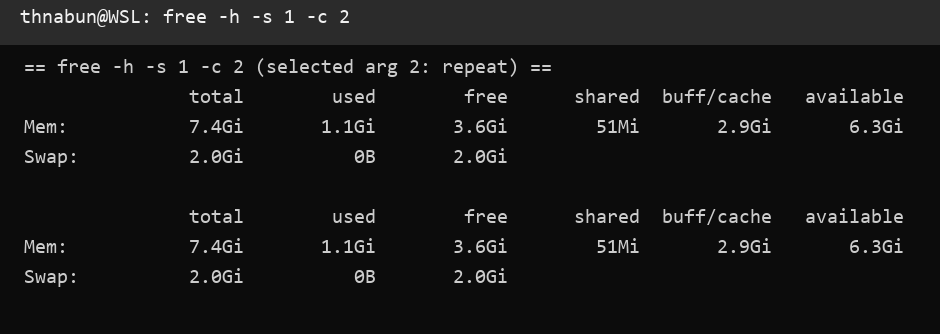
\includegraphics[width=0.95\linewidth]{free_repeat.png}
\caption{\texttt{free -h -s 1 -c 2} (repeat every 1\,s, twice).}
\end{figure}
\textbf{(2) \texttt{-s N -c N / --seconds --count}:} repeats printing every $N$ seconds, $N$ times. Sample: \texttt{free -h -s 1 -c 2} prints twice one second apart, useful to watch memory change during a workload without running \texttt{watch}.

\subsection{\texttt{vmstat}}
\begin{figure}[H]\centering
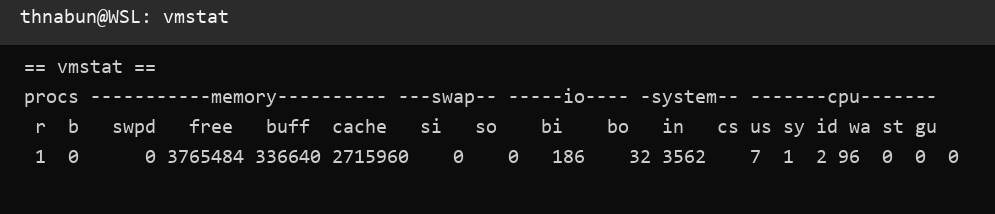
\includegraphics[width=0.95\linewidth]{vmstat.png}
\caption{\texttt{vmstat} capture (averages since boot + current sample).}
\end{figure}
Columns: \texttt{procs r/b} = runnable / uninterruptible processes; \texttt{memory swpd/free/buff/cache} (KiB swapped, free, buffers, page cache); \texttt{swap si/so} = swapped in/out per second; \texttt{io bi/bo} = blocks in/out; \texttt{system in/cs} = interrupts / context switches per second; \texttt{cpu us/sy/id/wa/st/gu} = user, system, idle, iowait, stolen, guest percent. First line after header is averages since boot; with \texttt{delay} the following lines are per-interval samples.

\textbf{Paragraph summary of values:} The snapshot shows no process pressure (0 runnable extra, 0 blocked, 0\,KiB swapped), about 3\,765\,484\,KiB free with 336\,640\,KiB buffers and 2\,715\,960\,KiB cache, zero swap-in/out, modest I/O (186 blocks in, 32 out), 3\,562 interrupts and 7 context switches per second on average, and CPU essentially idle at 1\% user, 2\% system, 96\% idle with 0\% iowait.

\subsection{Two useful \texttt{vmstat} arguments}
\begin{figure}[H]\centering
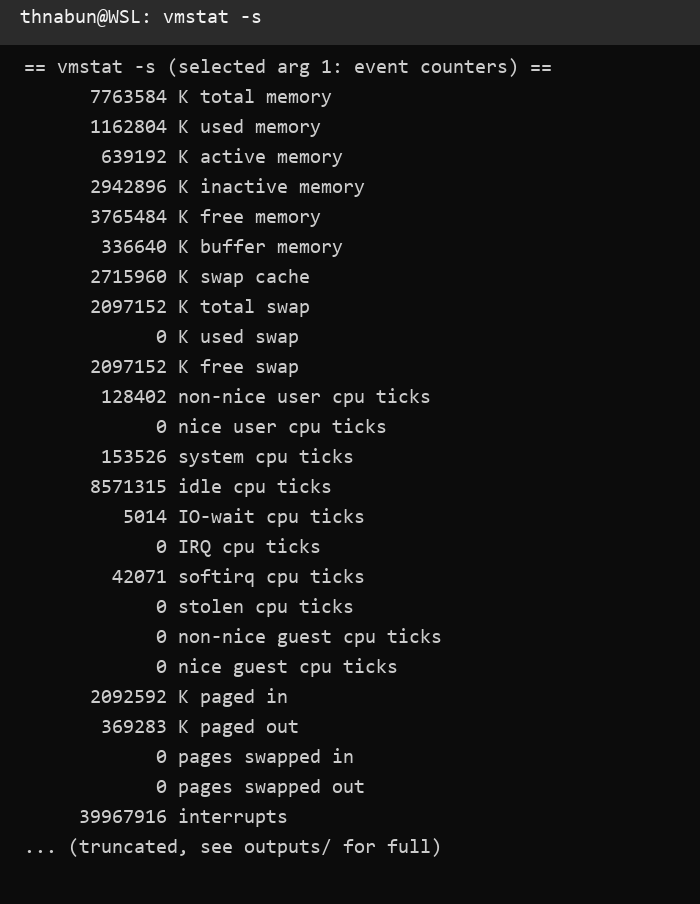
\includegraphics[width=0.75\linewidth]{vmstat_s.png}
\caption{\texttt{vmstat -s} (event counters, truncated in figure; full in \texttt{outputs/vmstat\_s.txt}).}
\end{figure}
\textbf{(1) \texttt{-s / --stats}:} prints absolute event counters instead of rates: total/used/active/inactive/free/buffer/swap-cache memory (here 7\,763\,584\,K total, 1\,162\,804\,K used, 3\,765\,484\,K free, 2\,097\,152\,K total swap all free), cpu ticks (128\,402 user, 153\,526 system, 8\,571\,315 idle), paging (2\,092\,592\,K paged in, 369\,283\,K out, 0 swapped), 39\,967\,916 interrupts, 64\,971\,497 context switches, 219\,325 forks since boot. Best for ``how much since boot'' questions.
\begin{figure}[H]\centering
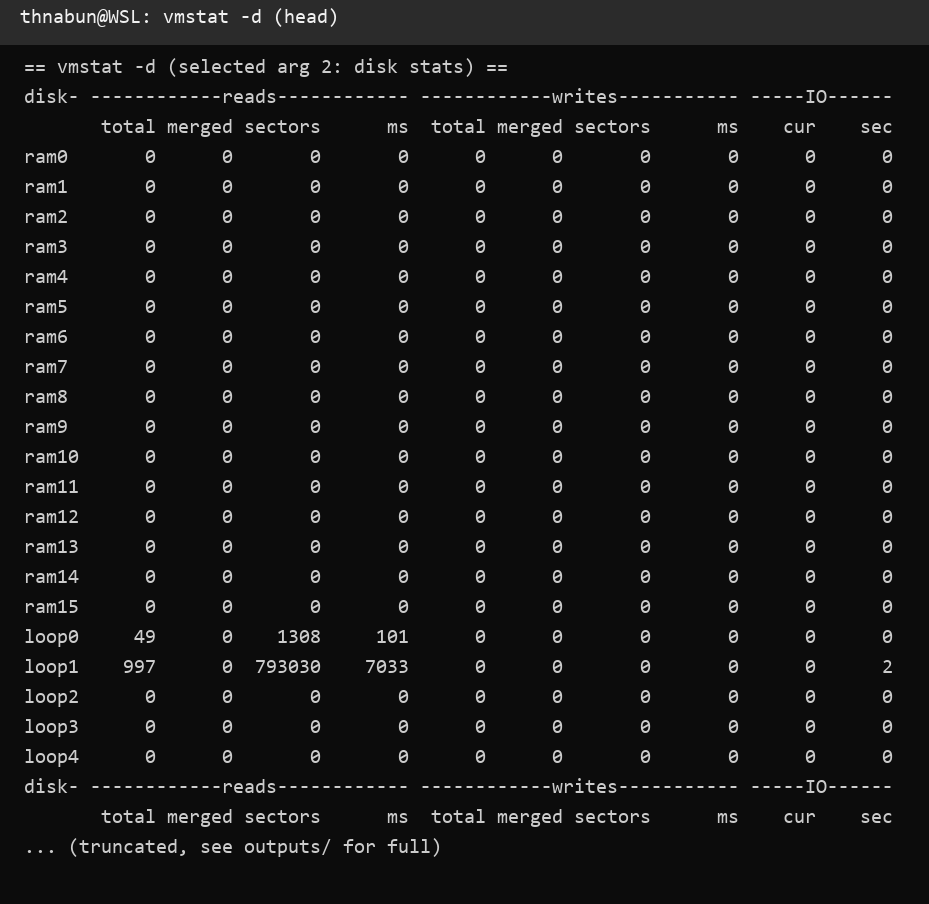
\includegraphics[width=0.75\linewidth]{vmstat_disk.png}
\caption{\texttt{vmstat -d} (disk stats, truncated; full in \texttt{outputs/vmstat\_d.txt}).}
\end{figure}
\textbf{(2) \texttt{-d / --disk}:} per-disk read/write totals, merges, sectors, milliseconds, and in-flight I/O. Here \texttt{sdd} dominates (51\,155 reads, 25\,903 writes), while \texttt{ram*/loop*} are near zero. Best to find which disk bottlenecks paging. Companion sampling form \texttt{vmstat 1 2} (one-second interval, two reports) shows the second line as current load (here 100\% idle), proving the first line is a since-boot average.

\section{Windows VM monitoring}
\subsection{Resource Monitor}
Open with \texttt{Win+R} $\rightarrow$ \texttt{resmon} (or PowerShell \texttt{resmon}), then the \texttt{Memory} tab (Overview also contains a Memory section). The interface shows per-process \texttt{Image, PID, Hard Faults/sec, Commit (KB), Working Set (KB), Shareable (KB), Private (KB)} plus right-side graphs (CPU, Disk, Network, Memory faults) and, on the Memory tab, a \texttt{Physical Memory} bar split into \texttt{In Use / Modified / Standby / Free} with a numeric \texttt{\% Used Physical Memory} header.
\begin{figure}[H]\centering
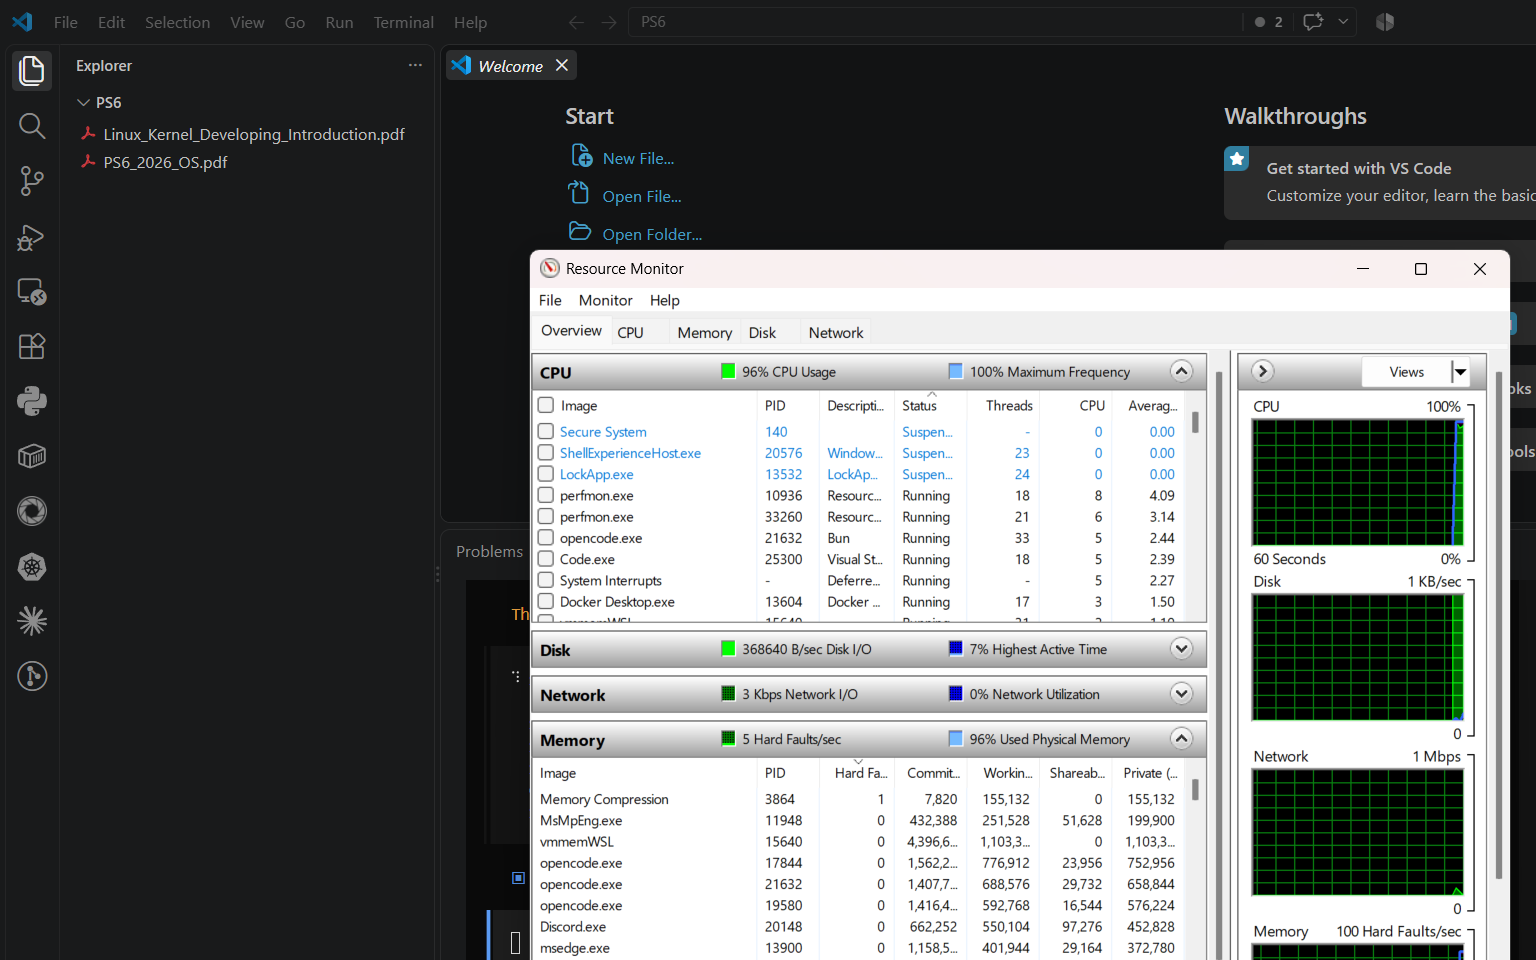
\includegraphics[width=0.95\linewidth]{resmon_memory.png}
\caption{Real \texttt{resmon} capture on this machine (Overview with Memory section expanded; Memory tab shows the same table plus the Physical Memory bar).}
\end{figure}
Meaning: \texttt{Hard Faults/sec} = pages fetched from disk (real I/O); \texttt{Commit} = private virtual committed; \texttt{Working Set} = resident; \texttt{Shareable/Private} split the working set; \texttt{96\% Used Physical Memory} here reflects a heavily loaded 16\,GB box; top consumers are \texttt{vmmemWSL}, \texttt{opencode.exe}, browsers/Discord, and \texttt{Memory Compression}.

\subsection{Physical-memory numbers (paragraph)}
Resource Monitor reported 96\% used physical memory with 5--107 hard faults/sec during capture. PowerShell corroboration (\texttt{Get-CimInstance Win32\_OperatingSystem}, \texttt{Win32\_PhysicalMemory}, \texttt{Get-Counter \textbackslash Memory\textbackslash*}): 16\,034\,164\,KB total visible ($\approx$15.3\,GiB) from 2$\times$8\,589\,934\,592-byte Kingston 5600 sticks, only $\approx$472\,200\,KB ($\approx$461\,MiB) free, 43\,297\,140\,KB total virtual with 7\,516\,852\,KB free, paging files holding 27\,262\,976\,KB with 23\,579\,072\,KB free, \texttt{C:\textbackslash pagefile.sys} peak usage 4\,099\,KB, committed bytes $\approx$36.5\,GB against a 44.3\,GB commit limit (82.4\% in use), available bytes $\approx$493\,MB, pool paged $\approx$791\,MB / nonpaged $\approx$1.42\,GB.
\begin{figure}[H]\centering
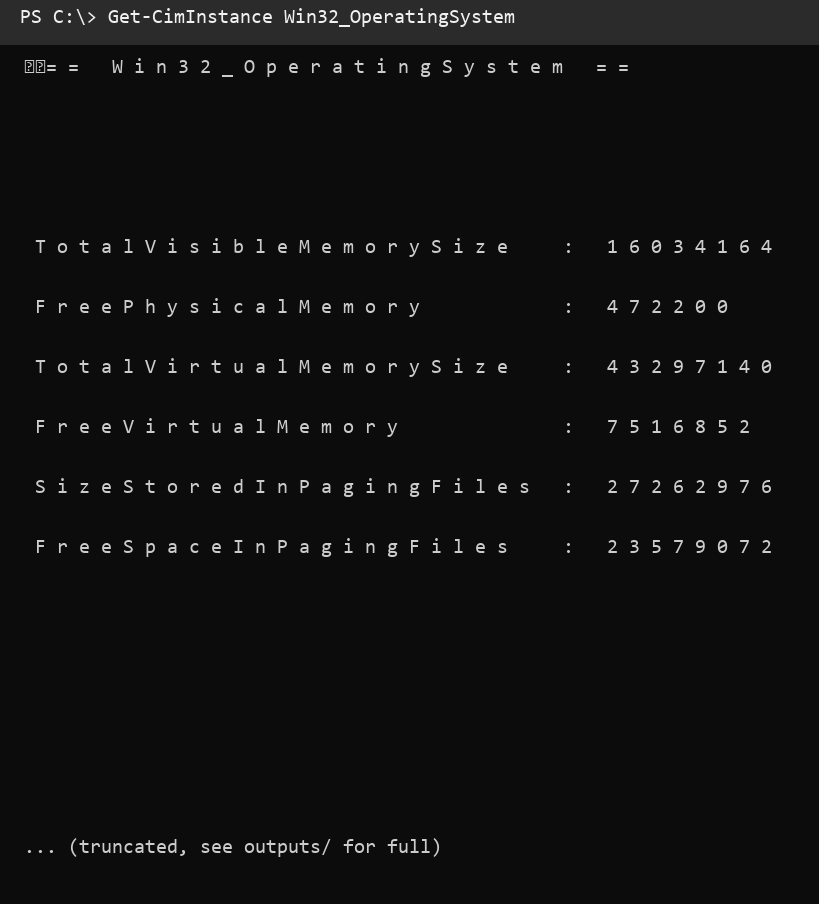
\includegraphics[width=0.85\linewidth]{windows_os.png}
\caption{\texttt{Get-CimInstance} memory + pagefile capture (see \texttt{outputs/windows\_os.txt}).}
\end{figure}

\section*{Appendix: reproduce}
\begin{lstlisting}[caption={Reproduce all captures}]
# Linux (WSL, in /home/thnabun/CPE333_OS/ps6)
bash scripts/linux_collect.sh
# swap demo (sudo will prompt for password)
bash scripts/swap_demo.sh
# Windows (PowerShell)
powershell -ExecutionPolicy Bypass -File scripts/windows_collect.ps1
# then Win+R -> resmon -> Memory tab -> screenshot to report/figures/
\end{lstlisting}

\end{document}
